\documentclass[pdftex,12pt,a4paper]{article}

\usepackage{graphicx}  
\usepackage[margin=2.5cm]{geometry}
\usepackage{breakcites}
\usepackage{indentfirst}
\usepackage{pgfgantt}
\usepackage{pdflscape}
\usepackage{float}
\usepackage{epsfig}
\usepackage{epstopdf}
\usepackage[cmex10]{amsmath}
\usepackage{stfloats}
\usepackage{multirow}

\renewcommand{\refname}{REFERENCES}
\linespread{1.3}

\usepackage{mathtools}
%\newcommand{\HRule}{\rule{\linewidth}{0.5mm}}
\thispagestyle{empty}
\begin{document}
\begin{titlepage}
\begin{center}
\textbf{}\\
\textbf{\Large{ISTANBUL TECHNICAL UNIVERSITY}}\\
\vspace{0.5cm}
\textbf{\Large{COMPUTER ENGINEERING DEPARTMENT}}\\
\vspace{2cm}
\textbf{\Large{BLG 242E\\ DIGITAL CIRCUITS LABORATORY\\ EXPERIMENT REPORT}}\\
\vspace{2.8cm}
\begin{table}[ht]
\centering
\Large{
\begin{tabular}{lcl}
\textbf{EXPERIMENT NO}  & : & 1 \\
\textbf{EXPERIMENT DATE}  & : & 18.03.2022 \\
\textbf{LAB SESSION}  & : & FRIDAY - 10.30 \\
\textbf{GROUP NO}  & : & G22 \\
\end{tabular}}
\end{table}
\vspace{1cm}
\textbf{\Large{GROUP MEMBERS:}}\\
\begin{table}[ht]
\centering
\Large{
\begin{tabular}{rcl}
150200056  & : & Furkan Salık \\
150160731  & : & Mustafa Cihad Günay \\
\end{tabular}}
\end{table}
\vspace{2.8cm}
\textbf{\Large{SPRING 2022}}

\end{center}

\end{titlepage}

\thispagestyle{empty}
\addtocontents{toc}{\contentsline {section}{\numberline {}FRONT COVER}{}}
\addtocontents{toc}{\contentsline {section}{\numberline {}CONTENTS}{}}
\setcounter{tocdepth}{4}
\tableofcontents
\clearpage

\setcounter{page}{1}

\section{INTRODUCTION [10 points]}

\begin{itemize}
\item Analysis of boolean functions, and realization of them using integrated circuits.
\item Observation of various functions with different frequencies using oscilloscope.
\end{itemize}

\section{MATERIALS AND METHODS [40 points]}

\subsection{DIAGRAMS OF CIRCUITS}
\subsubsection{Experiment Part 1}

\begin{figure}[ht]
	\centering
	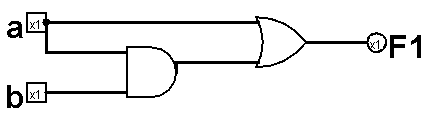
\includegraphics[width=0.5\textwidth]{f1_diagram.png}	
	\caption{Diagram of \(F_1(a, b) = a + a \cdot b\)}
	\label{fig1}
\end{figure}

\begin{figure}[ht]
    \centering
	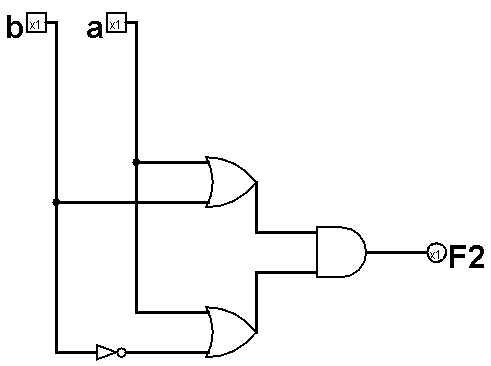
\includegraphics[width=0.5\textwidth]{f2_diagram.png}	
	\caption{Diagram of \(F_2(a, b) = a + a \cdot b\)}
	\label{fig2}
\end{figure}

\subsubsection{Experiment Part 2}
\begin{figure}[H]
	\centering
	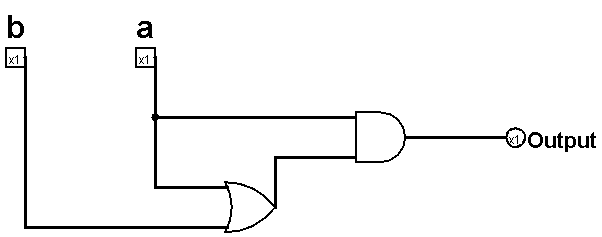
\includegraphics[width=0.5\textwidth]{part2_diagram.png}	
	\caption{Diagram of the dual of \(a + a \cdot b\), which is \(a \cdot (a + b)\)}
	\label{fig3}
\end{figure}

\subsubsection{Experiment Part 3}
\begin{figure}[H]
	\centering
	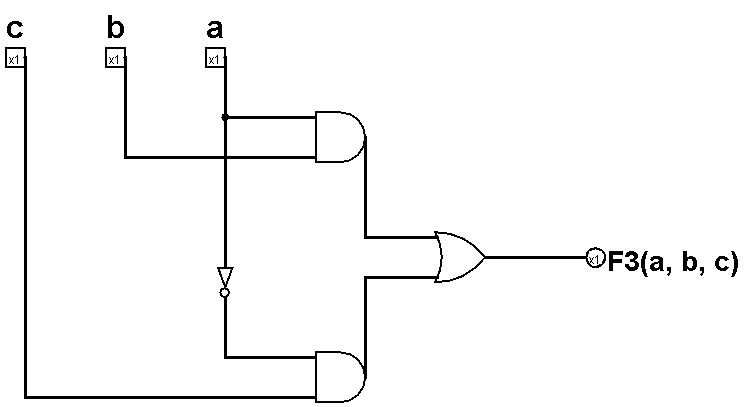
\includegraphics[width=0.5\textwidth]{f3_diagram.png}	
	\caption{Diagram of \(F_3(a, b, c) = a \cdot b + a' \cdot c\)}
	\label{fig4}
\end{figure}

\begin{figure}[H]
	\centering
	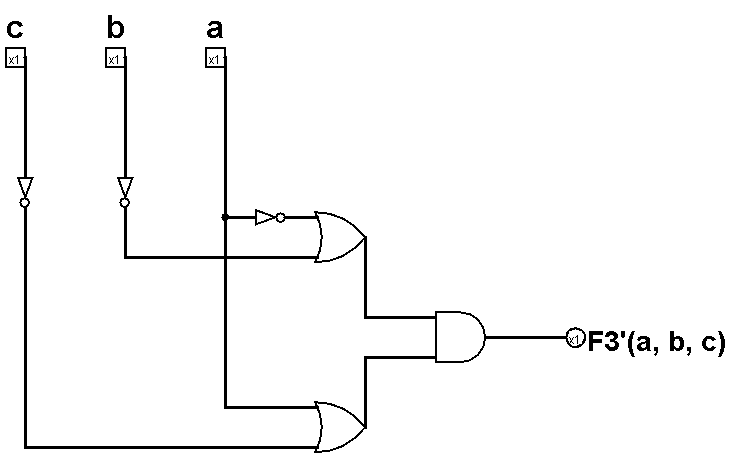
\includegraphics[width=0.5\textwidth]{f3_complement_diagram.png}	
	\caption{Diagram of \(\overline{F}_3(a, b, c) = (a' + b') \cdot (a + c')\)}
	\label{fig5}
\end{figure}

\subsubsection{Experiment Part 4}
\begin{figure}[H]
	\centering
	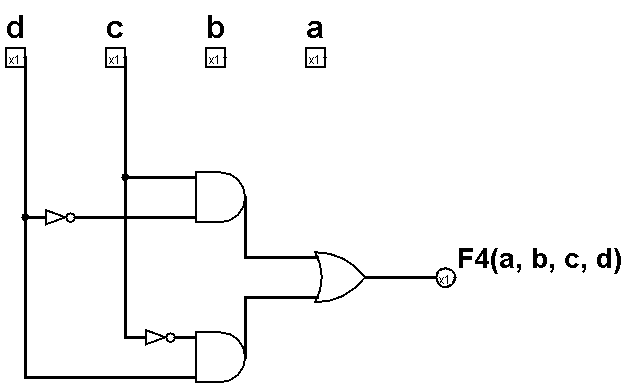
\includegraphics[width=0.5\textwidth]{f4_diagram.png}	
	\caption{Diagram of the simplified \(F_4(a, b, c, d) = c \cdot d' + c' \cdot d\)}
	\label{fig6}
\end{figure}

\subsection{THEORETICAL BACKGROUND}
\subsubsection{Experiment Part 2}
Dual of the theorem \(a + a \cdot b = a\) is \(a \cdot (a + b) = a\). We get this result by changing ORs to ANDs, and ANDs to ORs. If there were 0s or 1s, we would also invert them.

\subsubsection{Experiment Part 3}
Complement of the function \(F_3(a, b, c) = a \cdot b + a' \cdot c\) is \(\overline{F}_3(a, b, c) = (a' + b') \cdot (a + c')\). We get this result by applying De Morgan's Theorem.

\subsubsection{Experiment Part 4}
First of all, the function must be obtained. We note that the function is given in sums of products form, and we form the truth table:

\begin{figure}[H]
	\centering
	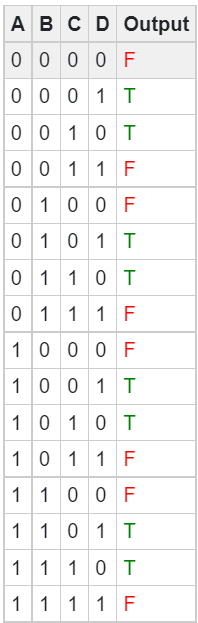
\includegraphics[width=0.28\textwidth]{f4_truthtable.PNG}	
	\caption{Binary representations of given indexes are assigned as true.}
	\label{fig7}
\end{figure}

After forming the truth table, we must form the Karnaugh Map. We place the true indexes as follows:

\begin{figure}[H]
	\centering
	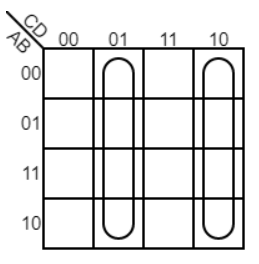
\includegraphics[width=0.4\textwidth]{f4_kmap.png}	
	\caption{It can be clearly seen that the simplified form is \(c \cdot d' + c' \cdot d\)}
	\label{fig8}
\end{figure}

\section{RESULTS [15 points]}
\begin{figure}[H]
	\centering
	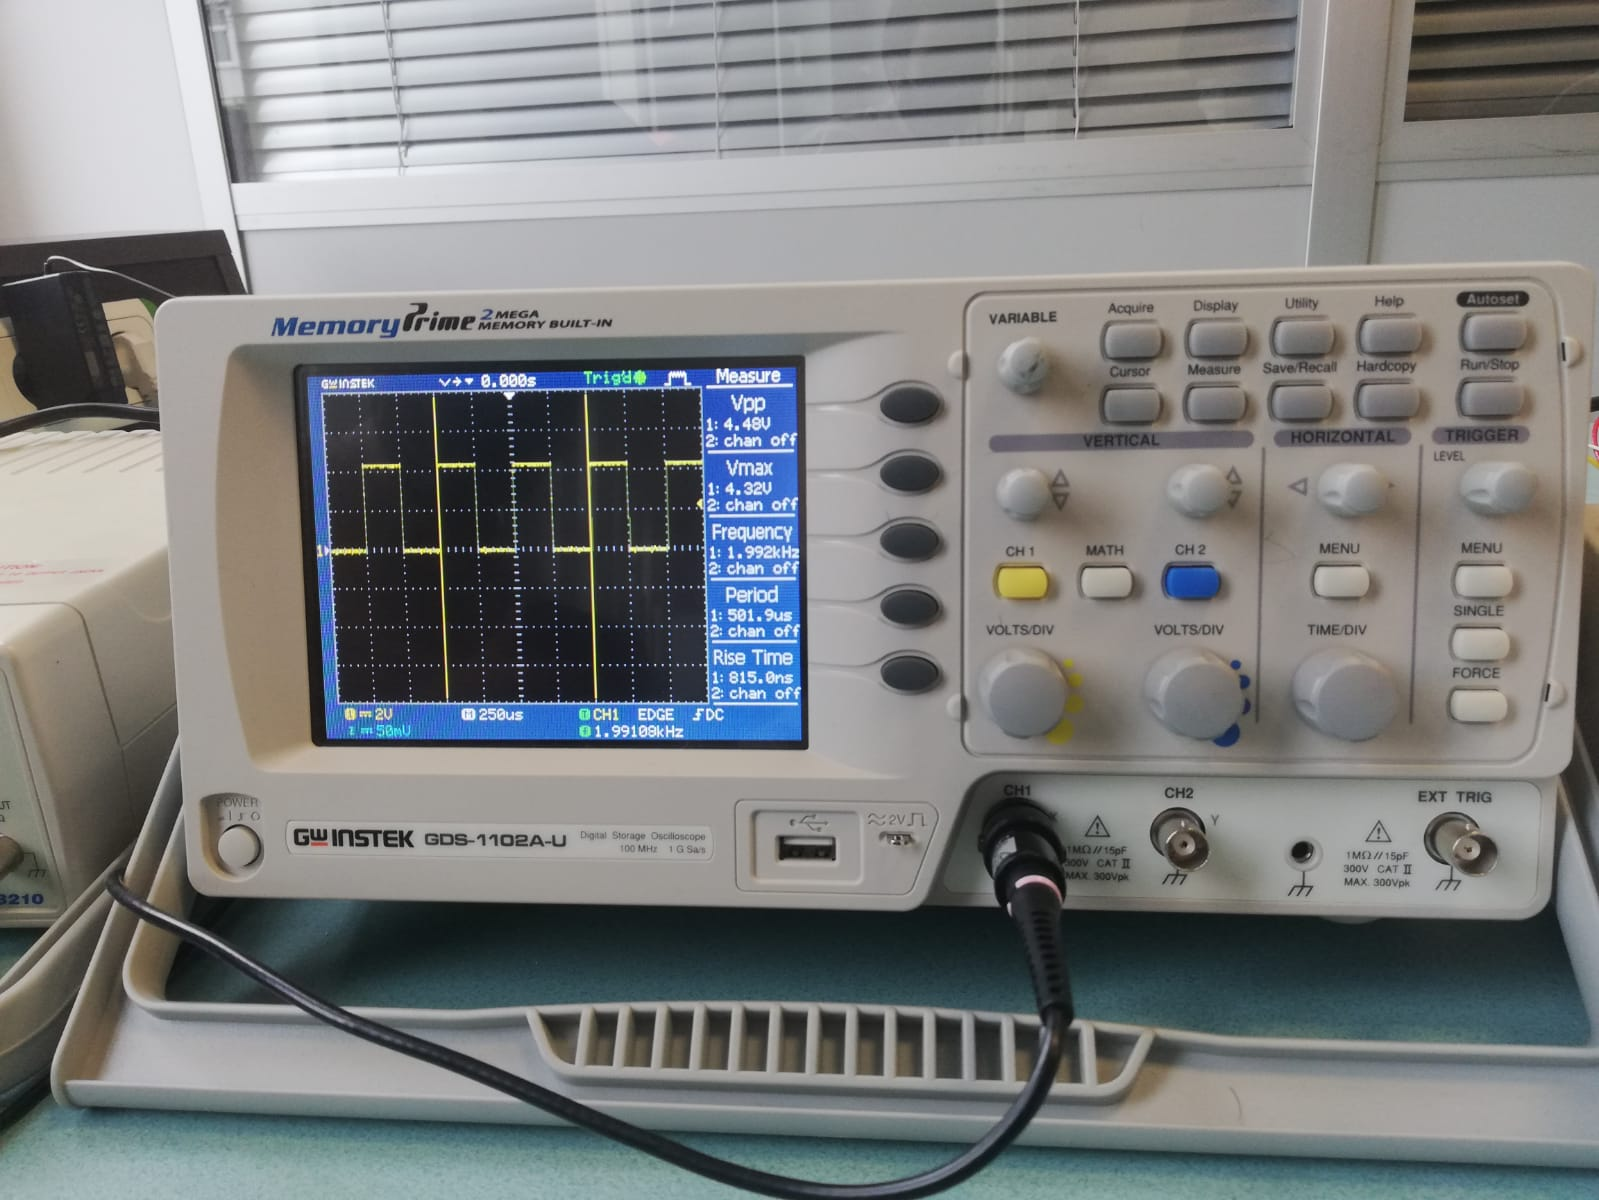
\includegraphics[width=0.85\textwidth]{osc1.jpg}	
	\caption{1992 Hz input.}
	\label{fig9}
\end{figure}

\begin{figure}[H]
	\centering
	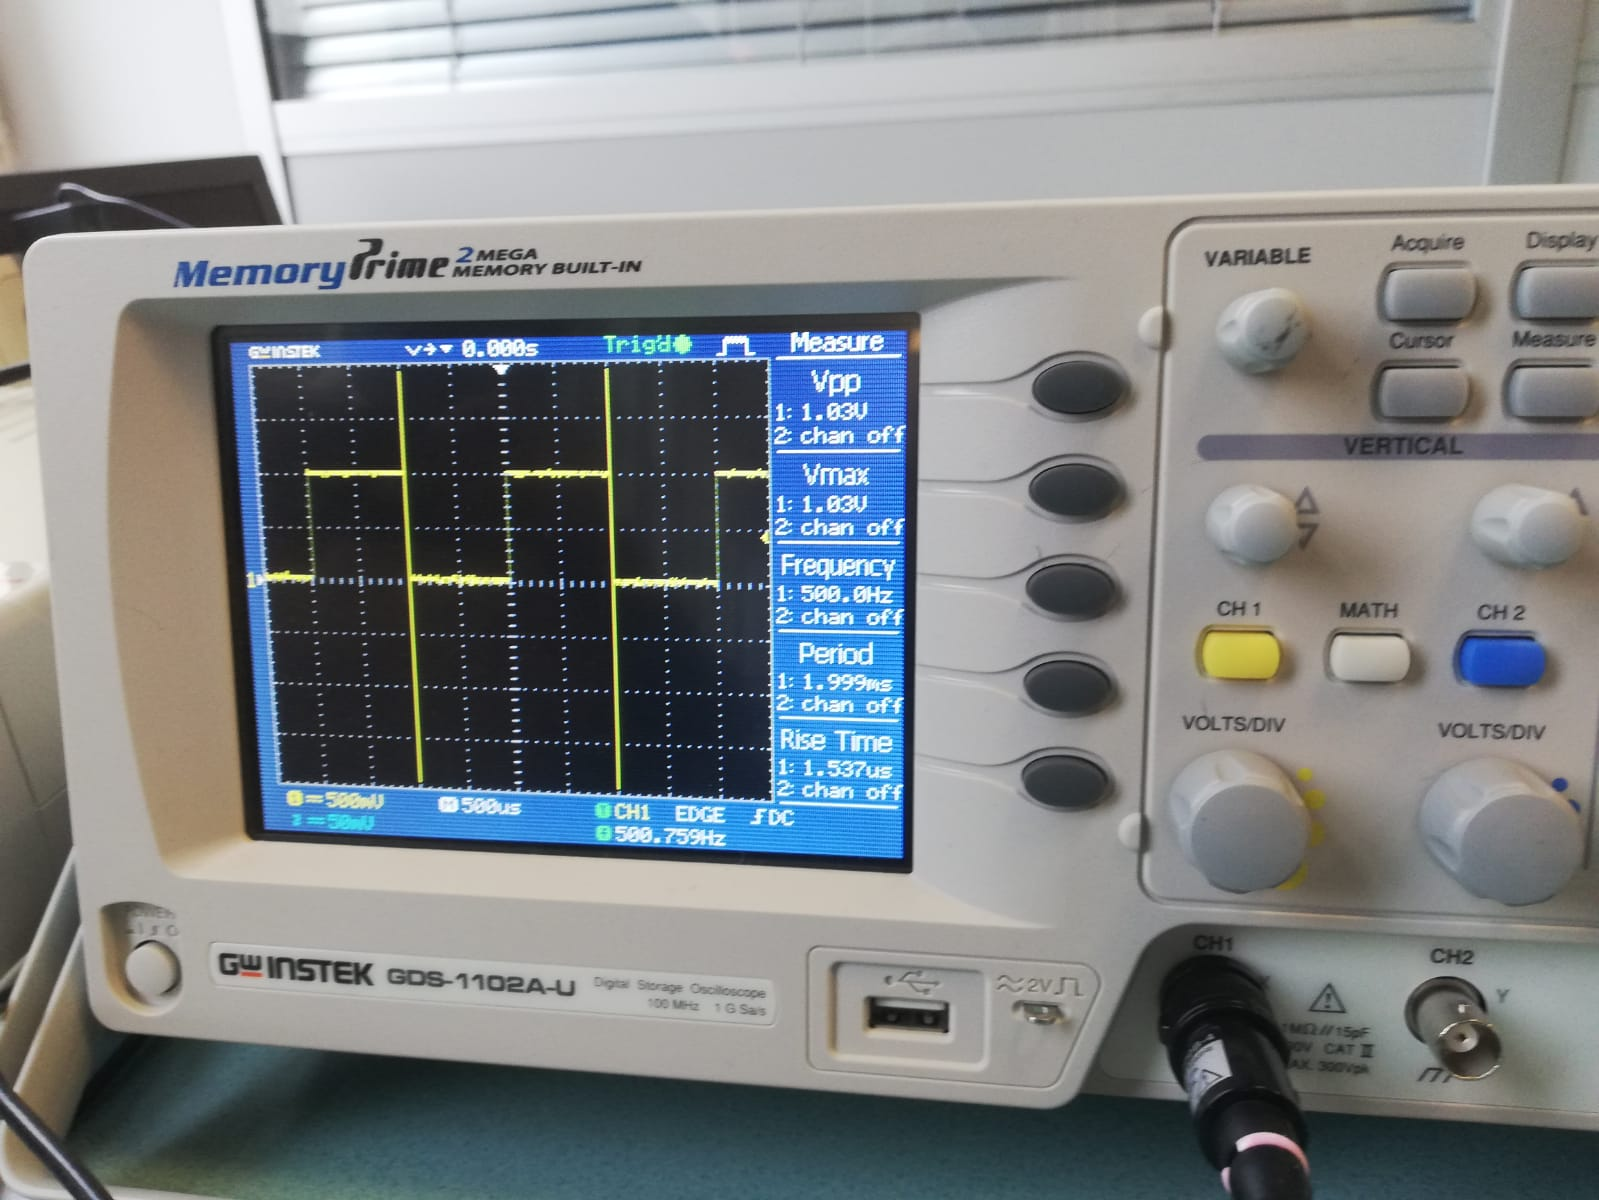
\includegraphics[width=0.85\textwidth]{osc2.jpg}	
	\caption{1 V, 500 Hz input.}
	\label{fig10}
\end{figure}

\begin{figure}[H]
	\centering
	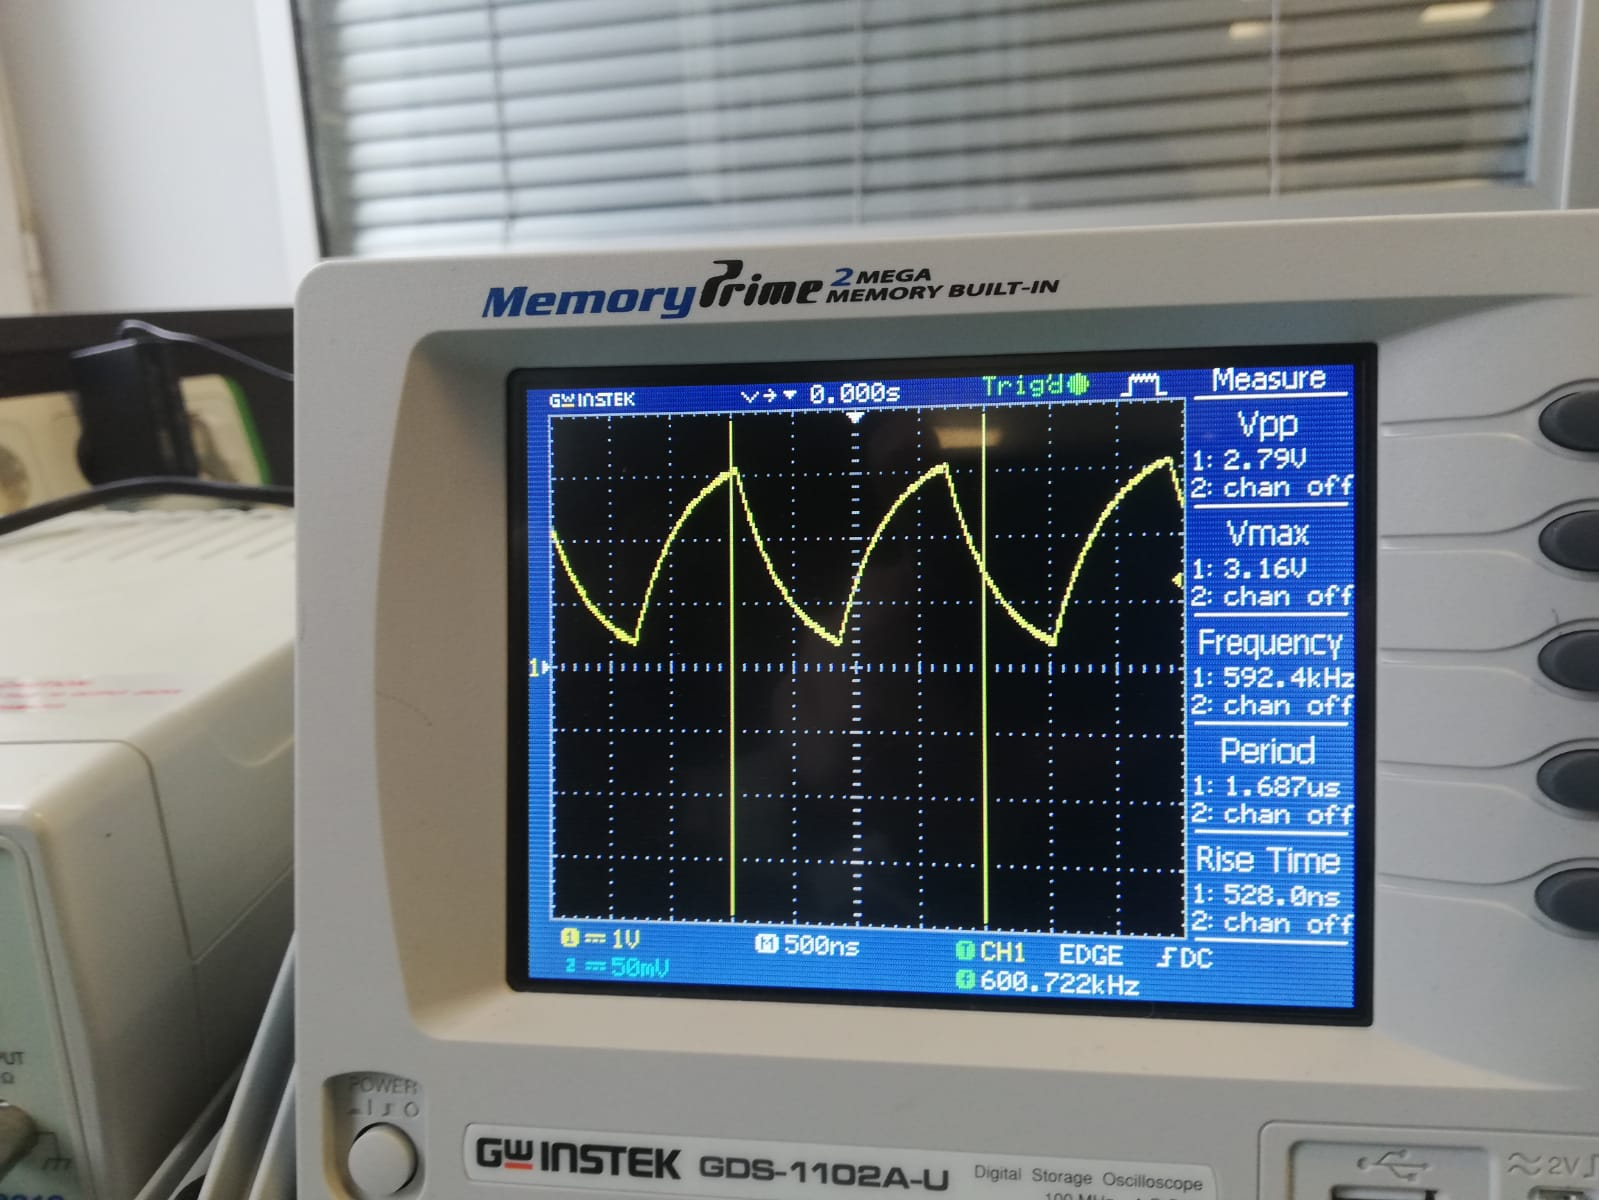
\includegraphics[width=0.85\textwidth]{osc3.jpg}	
	\caption{3.14 V, 0.6 MHz input.}
	\label{fig11}
\end{figure}

\begin{figure}[H]
	\centering
	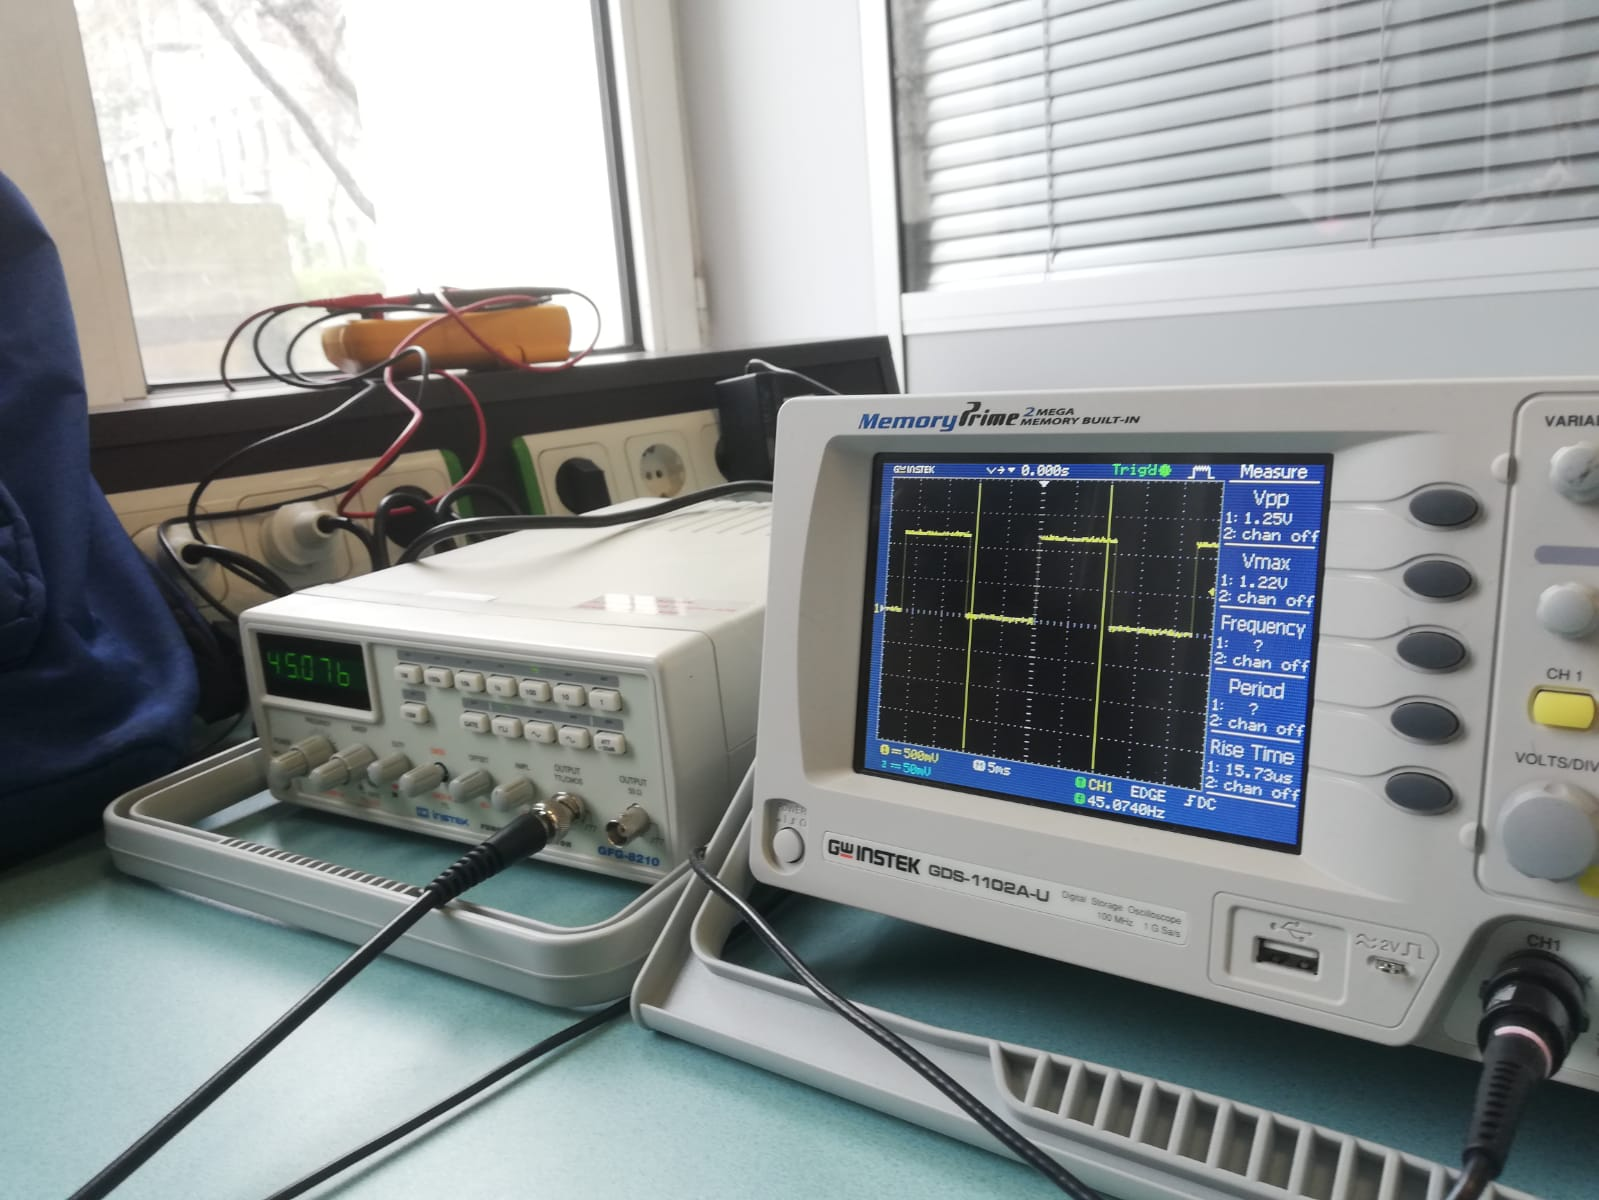
\includegraphics[width=0.85\textwidth]{osc4.jpg}	
	\caption{1.2 V input.}
	\label{fig12}
\end{figure}

\begin{figure}[H]
	\centering
	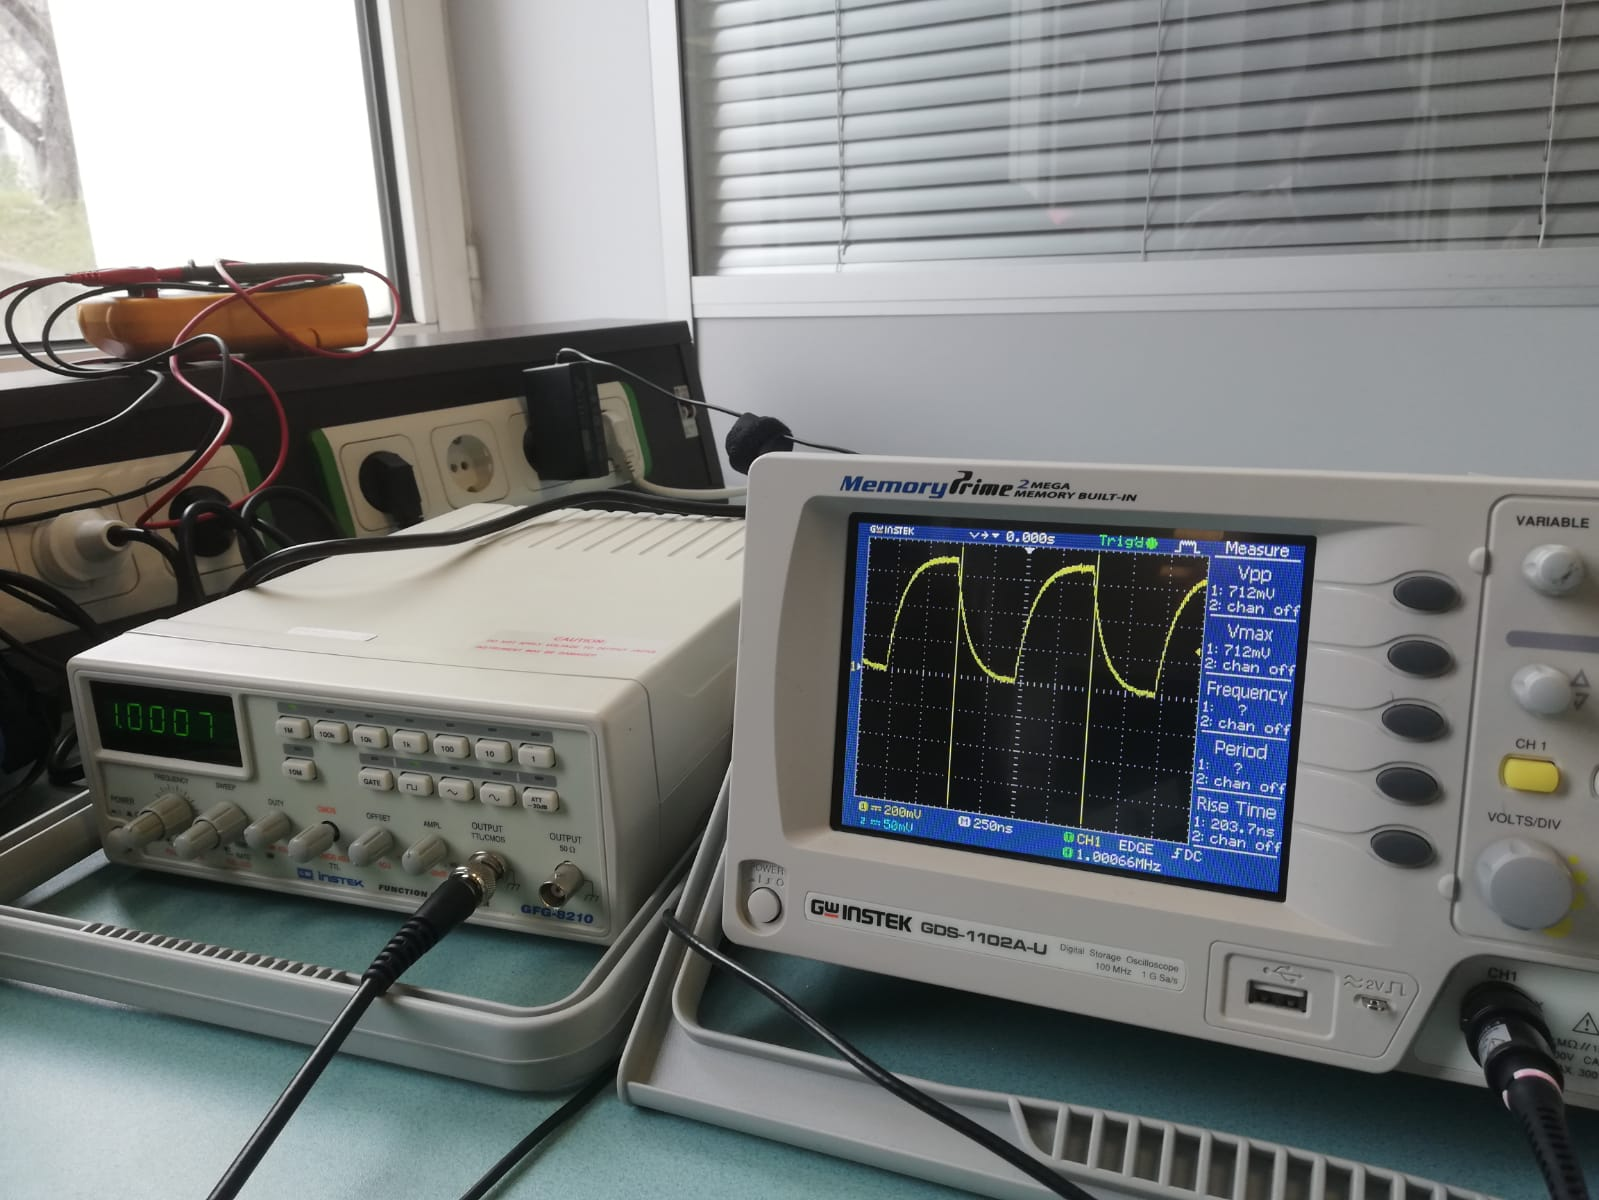
\includegraphics[width=0.85\textwidth]{osc5.jpg}	
	\caption{0.7 V input.}
	\label{fig13}
\end{figure}

\begin{figure}[H]
	\centering
	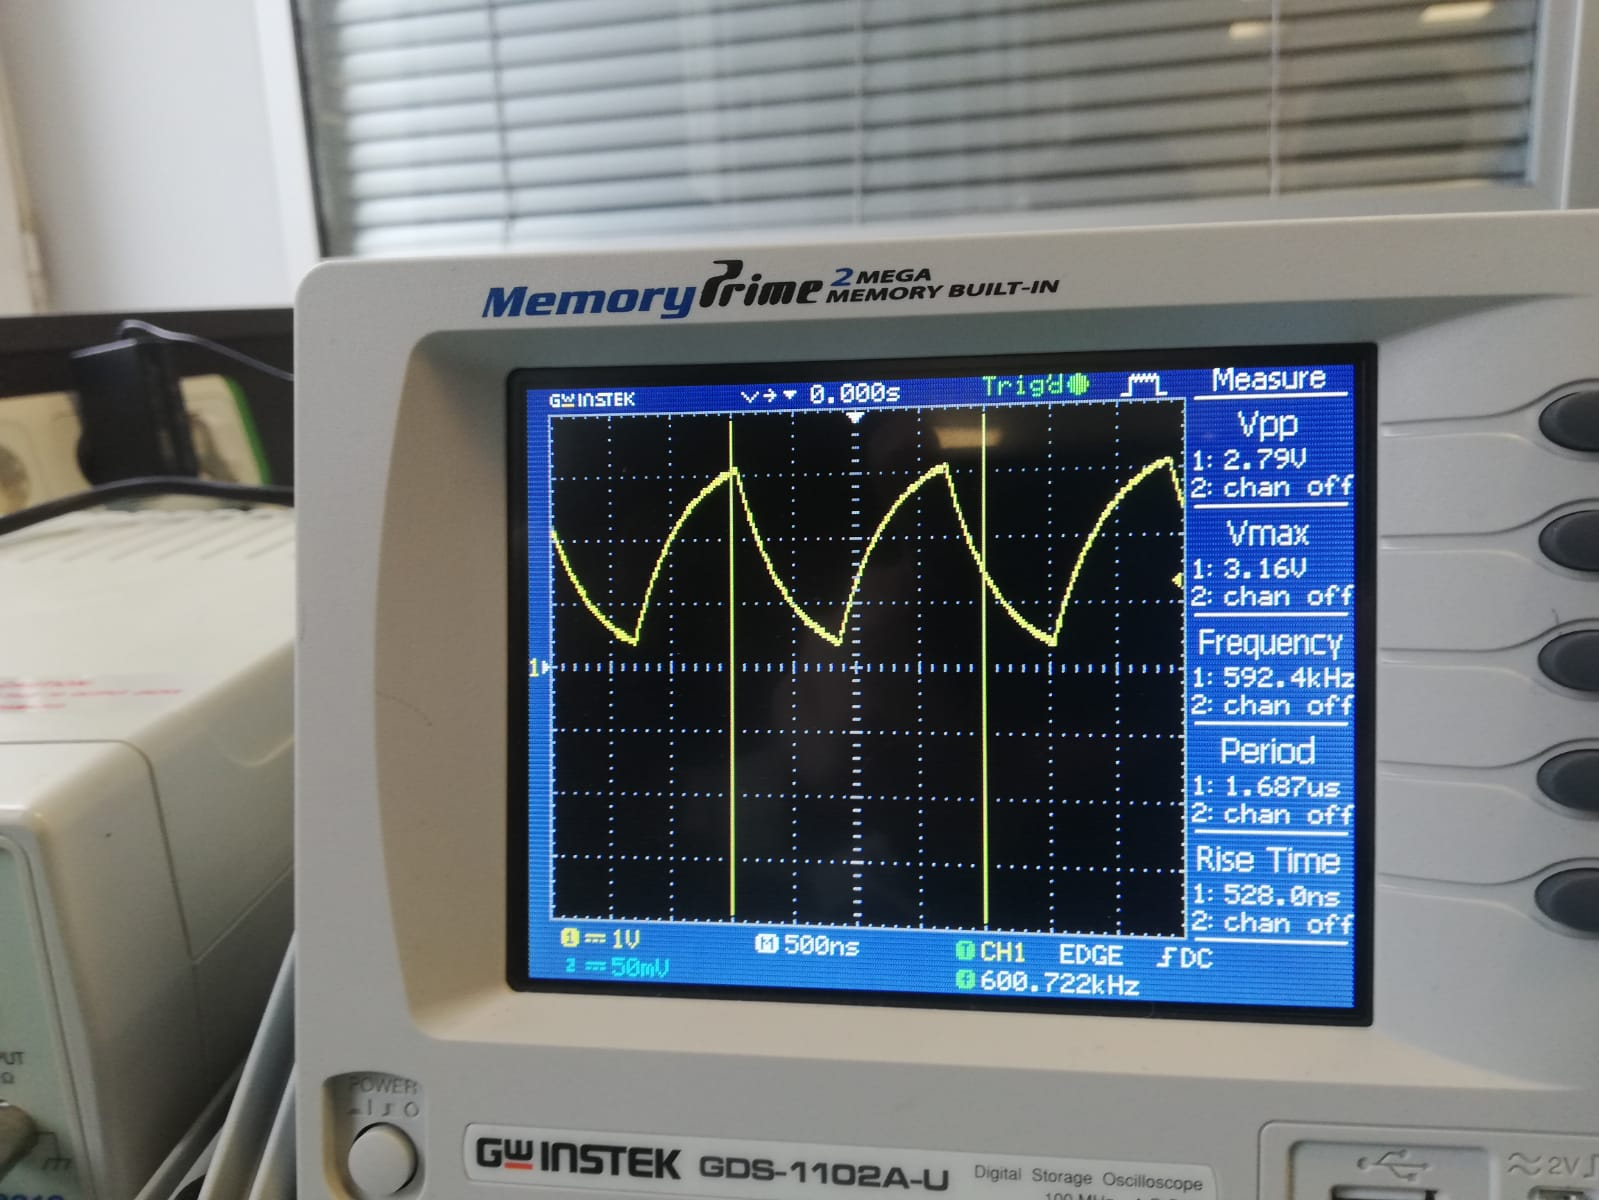
\includegraphics[width=0.85\textwidth]{osc3.jpg}	
	\caption{1250 mV input.}
	\label{fig14}
\end{figure}

\section{DISCUSSION [25 points]}
We first formed a theoretical base, i.e. used the properties and theorems of Boolean algebra. Then, we implemented the asked functions using logic gates. CADET was so useful for these experiments. It made our tasks easier, for example managing inputs, checking outputs and creating connections was so simple. Then, in another type of experiment, we observed the graphs of functions in various properties, such as frequency, period, voltage. Function generator and oscilloscope were the tools we used for this observation.

\section{CONCLUSION [10 points]}
Even though the experiments teached us many things related to electronics, we had some difficulties. Although CADET eased our tasks, there were malfunctioning parts of it, such as LEDs. We also had a problem in one of the integrated circuits, which was not showing the '0' output.

We gained experience in realizing Boolean functions, facing some problems and solving them. Also, we did not know what an oscillator and a function generator was before this experiment.

\newpage
\addcontentsline{toc}{section}{\numberline {}REFERENCES}

\bibliographystyle{unsrt}
\bibliography{reference}

\end{document}

